
\section{Evaluation}
\label{sec:5_eval}
% approx. 400-800 words
% \begin{itemize}
%     \item \textit{The metrics you used}
%     \item \textit{Results on evaluation that you performed}
%     \item \textit{Comparison and differences between you model and the baseline}
%     \item \textit{Correct interpretation of errors and analysis}
% \end{itemize}
\subsection{Metrics}
In this work we are framing the learning problem as a multi-class classification problem, where the classes to predict are the words in the vocabulary. Hence, we are training the model to minimize the cross-entropy (CE) loss:
\begin{equation}
    \text{CE} \parenth[\big]{f(x; \theta), y} = -\sum_{i=1}^{N} y_i \log{f(x_i; \theta)}
\end{equation}
where $f(x; \theta)$ is the model, $x$ is the input sequence, $y$ is the target sequence, $\theta$ is the set of model parameters and $N$ is the number of classes in the vocabulary. 

The main metric we used to compare and evaluate the models is the \emph{perplexity} (PP). The reason is that PP is a well understood and established metric and it correlates well enough with the model performances on real-world tasks. Although the PP can be defined in multiple ways, it is convenient to use the definition of PP as the exponential of the cross-entropy (CE):
\begin{equation}
    \text{PP}(f(x; \theta), y) = \exp \parenth[\big]{CE(f(x; \theta), y)}
\end{equation}

% Intuitively, the PP can be interpreted as the number of classes that the model is considering to make a prediction . 
While the $CE$ gives a measure of how much the model is uncertain about the prediction, the PP can be interpreted as a measure of how many classes the model is considering to make a prediction (\emph{weighted branching factor}). The lower the PP, the less uncertain the model is on which word to predict, the better it is performing.

Additionally, we are further evaluating the best-performing model to excerpt deeper insights in its behaviour. Specifically, we are considering \emph{average PP per sequence length}, \emph{per word predicted vs. target counts difference} and \emph{precision, recall} and \emph{F1 score}. Lastly, we are giving a qualitative evaluation of the model by showing some examples of generated sequences.

\subsection{Results}
We evaluated every model by performing an evaluation epoch on the \emph{validation} and \emph{test} set with batch size $1$. The results of these evaluation runs are summarized in Tab.\ref{tab:results}.
\begin{table}
    \begin{tabular}{lcc}
    \toprule
    \textbf{Model}& \textbf{Validation} & \textbf{Test} \\
    \midrule
    \texttt{baseline\_dropout} & 116.11 & 113.44 \\
    \texttt{merity\_ad} & 95.36 & 	91.29 \\
    \texttt{merity\_ad\_nohh} & 95.36 & 91.29 \\
    \texttt{merity\_ad\_nohh\_tbptt} & 90.38 &	87.46 \\
    \texttt{merity\_ad\_nohh\_1024} & 85.85 &	82.74 \\
    \texttt{merity\_ad\_nohh\_1024\_ps} & 87.40 &	83.18 \\
    \texttt{merity\_ad\_nohh\_1024\_ps\_long} & 83.01 &	79.86 \\
    \bottomrule
\end{tabular}
    \caption{Results (PP) of the experiments.}
    \label{tab:results}
\end{table}
It is worth noting that we decided to scrap \emph{Weight Dropout} on the hidden-to-hidden weight matrices of the LSTM layers. The reason is that the the model with the three dropout techniques (\texttt{merity\_ad}) was achieving worse results than the model with only \emph{Variational Dropout} and \emph{Embedding Dropout} (\texttt{merity\_eld}), as it can be seen in Fig\ref{fig:tl_merity_ads}.

\begin{figure}
    \centering
    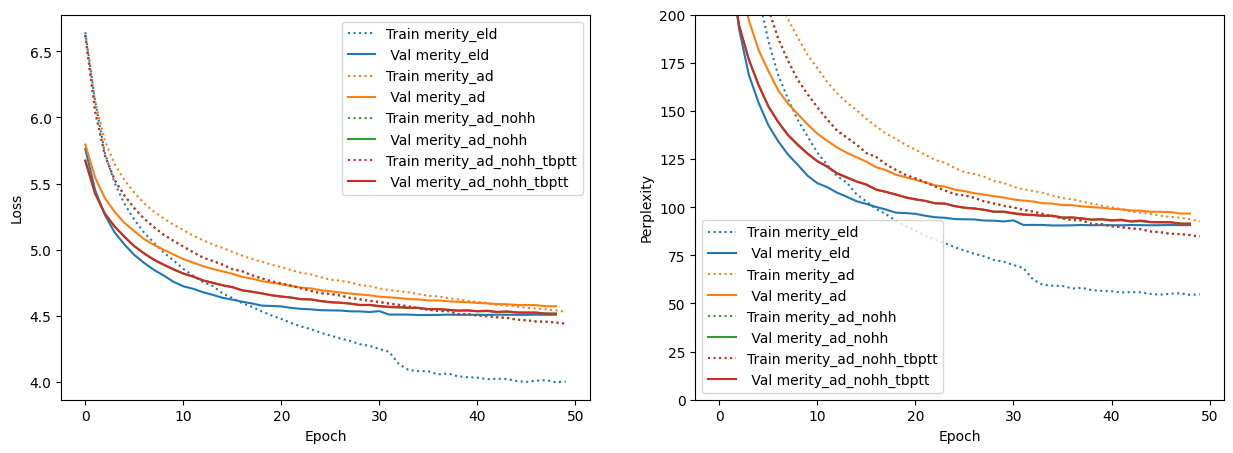
\includegraphics[width=\textwidth]{./assets/images/tl_merity_ads}
    \caption{Training and validation loss  and PP of the models with dombined dropout techniques. The \texttt{merity\_eld} model uses only \emph{Variational Dropout} and \emph{Embedding Dropout}, the \texttt{merity\_ad} model uses all the three dropout techniques and \texttt{merity\_ad\_nohh} removes dropout on the hidden-to-hidden weight matrices in Weight Dropout.}
    \label{fig:tl_merity_ads}
\end{figure}

Hence, we performed further experiments on the \texttt{merity\_wd} model. We found out that \texttt{merity\_wd\_nohh} was achieveng better results on the validation set, as in Fig\ref{fig:tl_merity_wd}. This behaviour is probably caused by the fact that dropping out the hidden-to-hidden weights prevents the model from effectively learn long-term dependencies in the sequences. In the end, we decided to keep the \texttt{merity\_ad\_nohh} model as it had the best performances and still little overfitting.
\begin{figure}
    \centering
    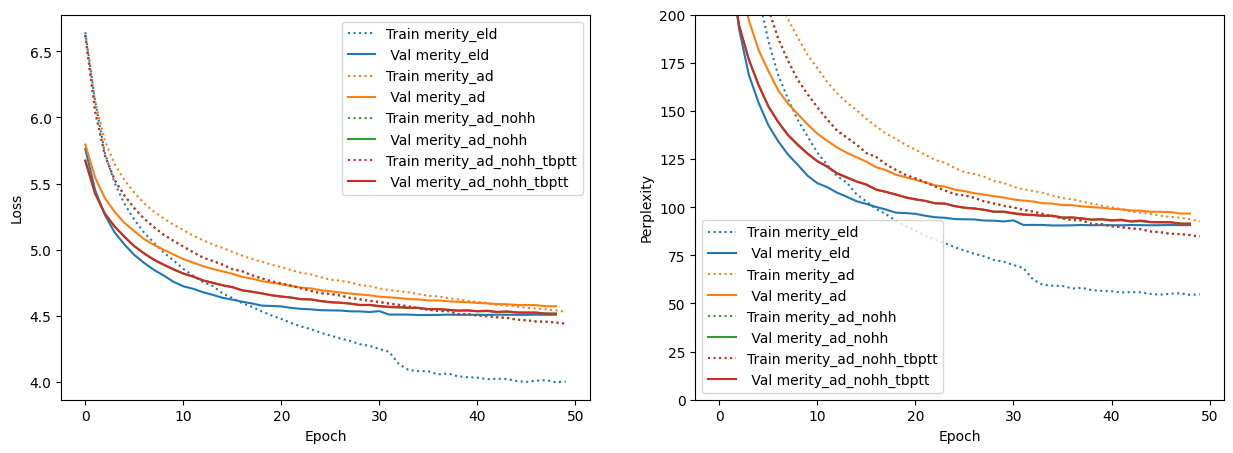
\includegraphics[width=\textwidth]{./assets/images/tl_merity_ads}
    \caption{Ablation study on \texttt{merity\_wd}.}
    \label{fig:tl_merity_wd}
\end{figure}

For similar reason we decided to discard TBPTT as training algorithm, as it was not improving the performances, and stick with unconstrained BPTT. On the other end, the models with increased embedding and hidden sizes achieved better results; we also reduced the number of LSTM layers from $3$ to $2$ and increased the probabilities of the dropout techniques to account for the increased model size. Similar considerations hold for the usage of \emph{Partial Shuffle}, which ensures less overfitting at the expensive of slightly higher PPs; the reason is that partially shuffling the sentences increases variety in the training data, acting as a sort of data augmentation technique. Lastly, we performed an extensive training experiment on the \texttt{merity\_ad\_nohh\_1024\_ps} model, where we let it train until the validation loss would stop decreasing at epoch $96$; this final and best performing model model scored $83.01$ PP on the validation set and $79.86$ on the test set.

\subsection{Analysis}